Hadoop è un framework di natura open-source sviluppato da Apache.
Obiettivo della piattaforma è la gestione, elaborazione e memorizzazione di grandi quantità di dati in modo scalabile.

Hadoop si pone come alternativa rispetto al modello \textit{Massively Parallel Processor (MPP)}.
In questo paradigma vengono impiegati più processori, ciascuno avente le proprie risorse di memoria e disco.
Il lavoro complessivo è suddiviso in task.
Ciascun task è poi eseguito da un processore a seconda delle politiche di schedulazione del sistema.
Le architetture MPP sono composte da hardware e software proprietari.ù

Al contrario Hadoop è progettato per operare su commodity hardware e software open-source.
Il commodity hardware è l'insieme di tutte le componenti hardware già in possesso di un utente.
Tali componenti sono spesso generiche e senza particolari specifiche.
Ciò permette di poter integrare anche risorse di natura e caratteristiche differenti tra loro, senza per forza dover mantenere un omogeneità all'interno del sistema.
Questa diversità, oltre ad abbattere i costi, consente tempi di manutenzione e sostituzione più veloci.

Il framework Hadoop si compone di quattro moduli principali:

\begin{itemize}
    \item \textbf{HDFS}.
    \textit{File system} distribuito con alto throughput e replicazione a livello di blocco.
    \item \textbf{MapReduce} Framework per la creazione di applicazioni in grado di processare grandi moli di dati. 
    MapReduce è pensato per astrarre la complessità della gestione parallela della computazione.
    Per l'utente è necessario solamente specificare le fasi di Map (elaborazione parallela sui dati) e di reduce (aggregazione dei risultati).
    \item \textbf{Common}. Questo modulo contiene librerie e strumenti di utilità per la gestione del sistema.
    \item \textbf{YARN}. Framework per la gestione delle risorse all'intero del cluster Hadoop.
\end{itemize}

Oltre a questi sono disponibili ulteriori moduli accessori, illustrati in~\cref{fig:chap-6:hadoop-modules}.

\begin{figure}
    \centering
    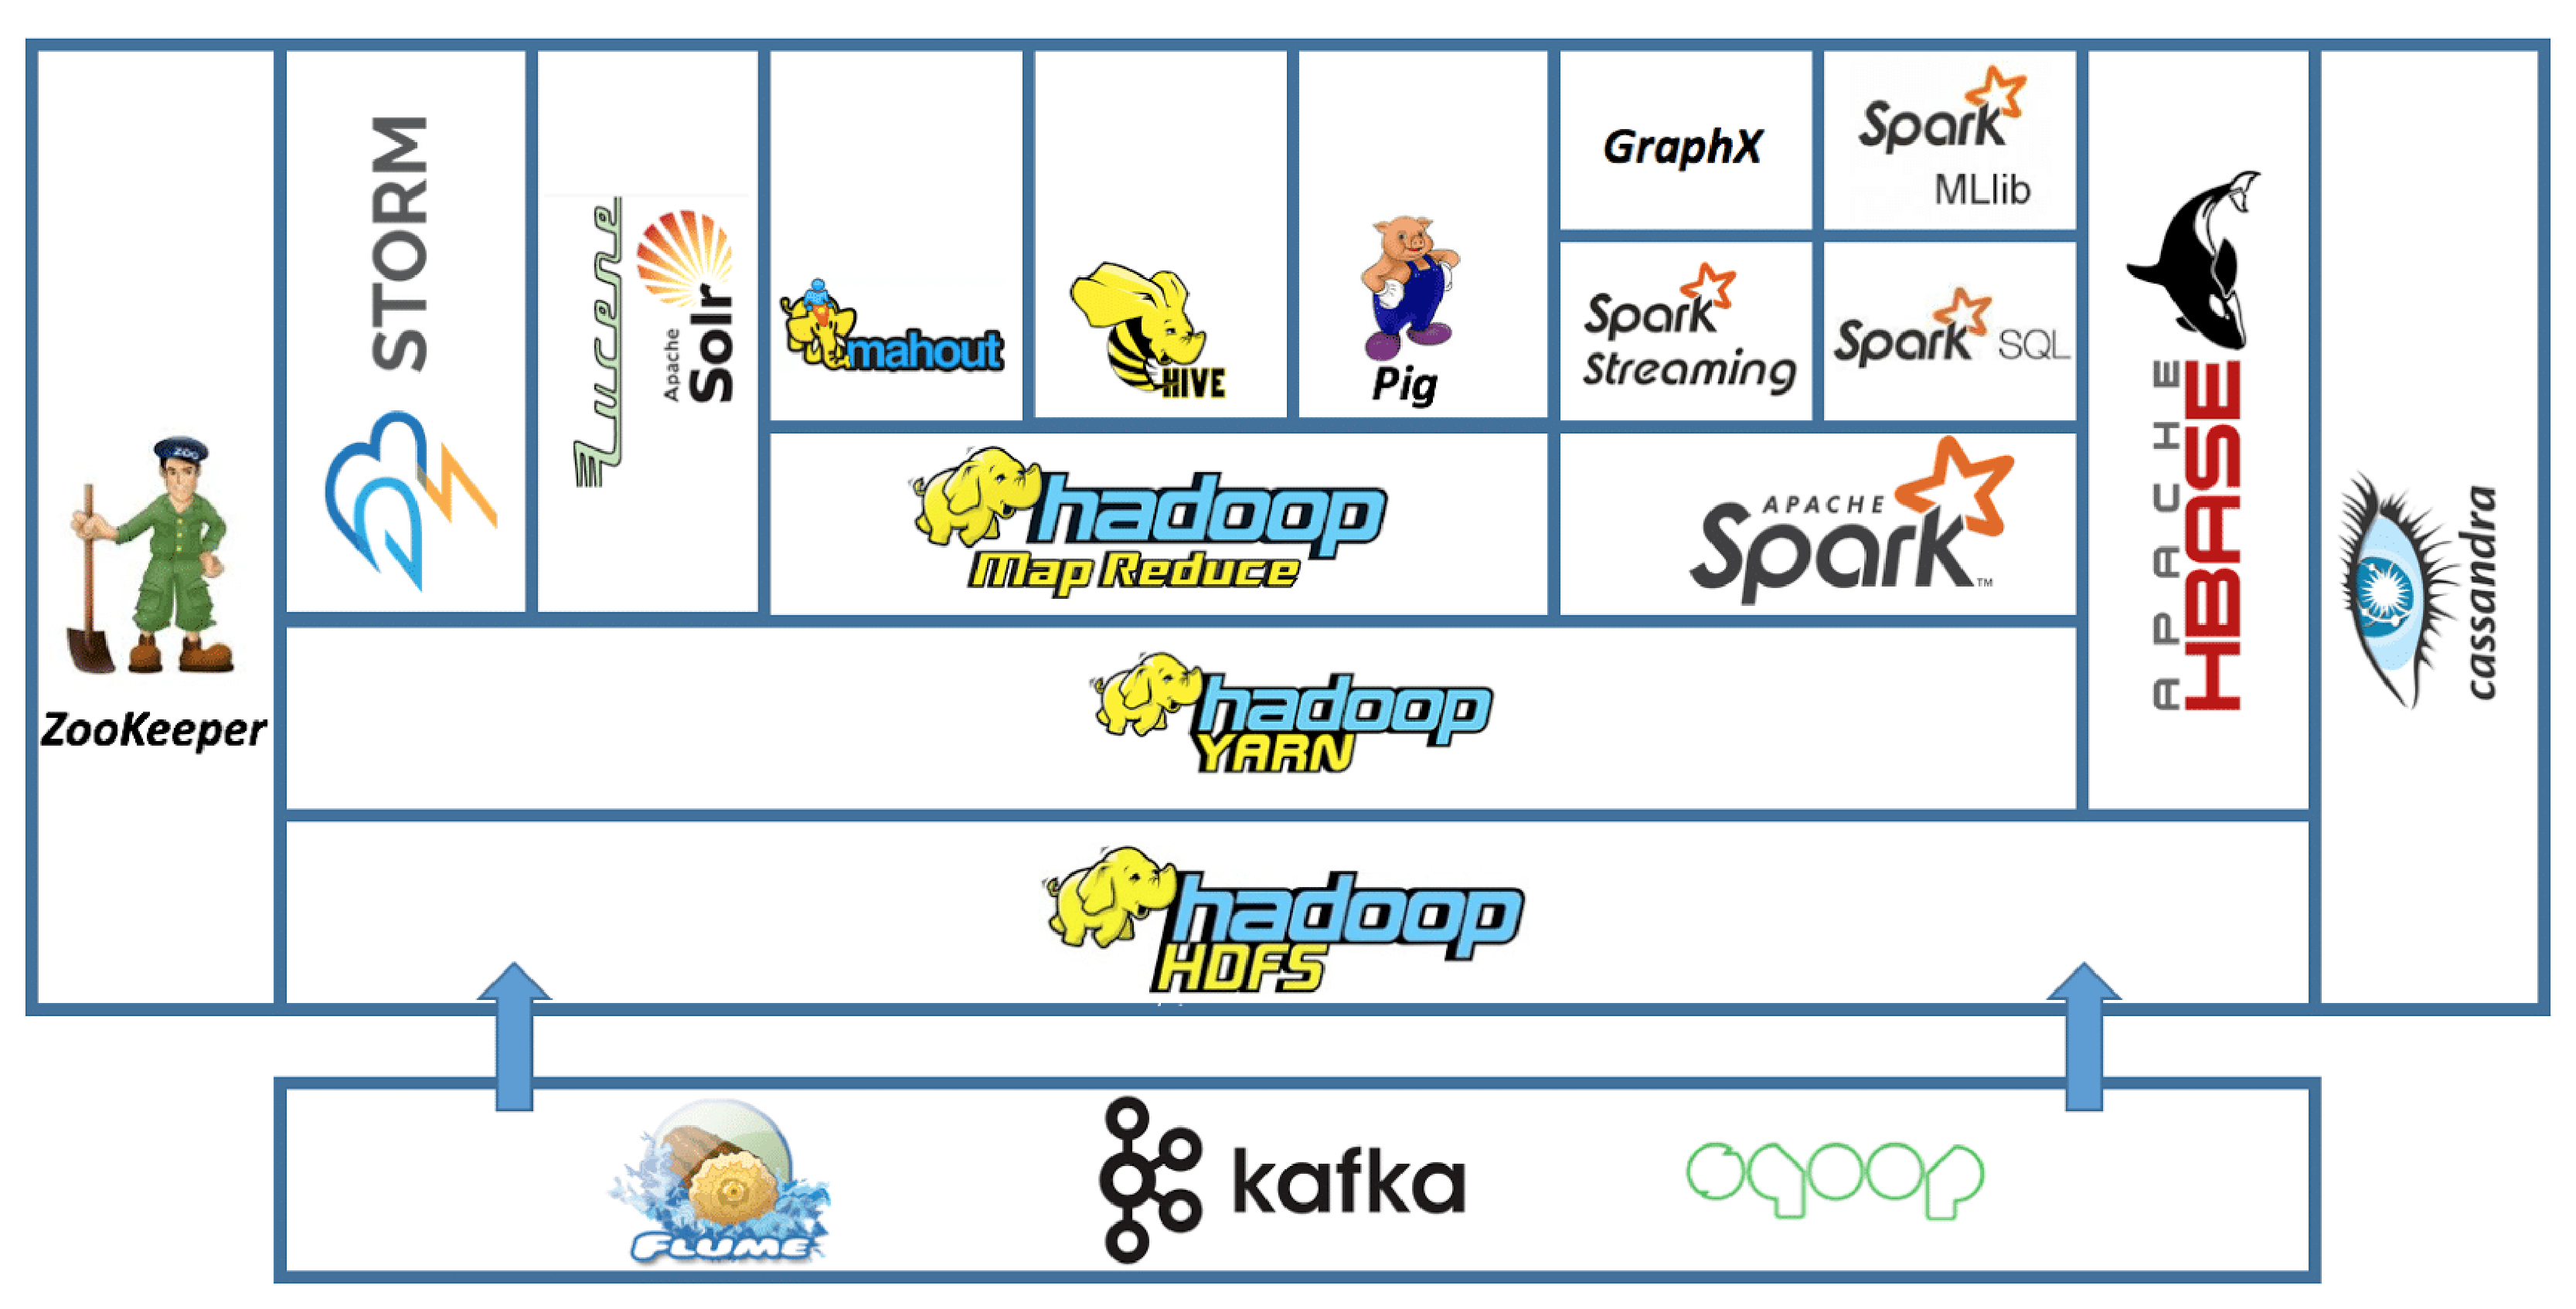
\includegraphics[width=\textwidth]{res/fig/sec-6/HadoopStack.pdf}
    \caption{Panoramica dell'ecosistema Hadoop, Fonte: \cite{Introduc53:online}}%
    \label{fig:chap-6:hadoop-modules}
\end{figure}